\documentclass[11pt,a4paper,oneside]{report}

\usepackage{amsmath,amssymb}
\usepackage{parskip}
\usepackage{graphicx}
\usepackage{xcolor}
\usepackage[a4paper,margin=1in]{geometry}
\usepackage{longtable,booktabs,array}

\usepackage{titlesec}
\titleformat{\chapter}[display]
  {\sffamily\bfseries\huge}
  {\Large \chaptertitlename\ \thechapter}
  {2ex}
  {\titlerule
  \vspace{1ex}%
  \filright\MakeUppercase}
  [\vspace{1ex}%
\titlerule]
\titleformat{\section} {\normalfont\sffamily\Large\bfseries} {\thesection}{1em}{}
\titleformat{\subsection} {\normalfont\sffamily\large\bfseries} {\thesubsection}{1em}{}
\titleformat{\subsubsection} {\normalfont\sffamily\normalsize\bfseries} {\thesubsubsection}{1em}{}
\usepackage[backend=biber, style=numeric-comp]{biblatex}
\addbibresource{bibfile.bib}

\usepackage[no-math]{fontspec}
\usepackage{unicode-math}
\defaultfontfeatures{Ligatures=TeX}
\setmainfont{Source Serif Pro}[BoldFont={Source Serif Pro Semibold}]
\setsansfont{SourceSansPro-Regular}[BoldFont={SourceSansPro-Semibold}]
\IfFontExistsTF{Cambria Math} {\setmathfont{Cambria Math}[Scale=1]} {\setmathfont{Asana Math}}

\usepackage{xeCJK}
\setCJKmainfont{Noto Sans SC}
\setCJKsansfont{Noto Sans SC}

\newcommand{\instructions}[1]{{\color{black}\itshape #1}}

\usepackage{upquote}
\usepackage[allcolors=blue,colorlinks=true]{hyperref}
\usepackage{xurl}
\usepackage{microtype}
\usepackage{bookmark}
\usepackage{calc}
\usepackage{etoolbox}

\usepackage{setspace}

\urlstyle{same}

\begin{document}

\onehalfspacing

% Author name (capitalized in its regular way)
\newcommand{\authorname}{Jingheng Huan}

% Title (cannot exceed three lines)
% You can insert manual linebreaks with \\
\newcommand{\thetitle}{A CASE STUDY OF AI IN VISION AND SOUND GENERATION: THE EVOLUTION, APPLICATIONS, AND ETHICAL CONSIDERATIONS}

% Date of submission with normal capitalization. 
% Use the format January 29, 2022.
\newcommand{\submissiondate}{Mar 7, 2024}

% Mentor: First Name Last Name (normal capitalization)
\newcommand{\mentor}{Peng Sun}

% Academic Unit (no abbreviations)
\newcommand{\academicunit}{Division of Natural and Applied Sciences}

%%%%%%%%%%%%%%%%%%%%%%%%%%%%%%%%%%%%%%%%%%%%%%%%%%%%%%%%%%%%%%%%%%%%%%%%%%%%%%%%

%% DO NOT CHANGE DIRECTLY THE CONTENTS OF THE TITLE PAGE.
%% TO CUSTOMIZE THE TITLE PAGE CHANGE THE DEFINITIONS OF THE COMMANDS
%% \authorname, \thetitle, \submissiondate, \mentor, \academicunit




\begin{titlepage}

\vspace*{\bigskipamount}

\begin{center}
{\sffamily\LARGE\bfseries\MakeUppercase\thetitle\par}

\bigskip

by

\bigskip

{\Large \authorname}

\bigskip

Signature Work Product, in partial fulfillment of the \\
Duke Kunshan University Undergraduate Degree Program

\bigskip

\emph{\submissiondate}

\bigskip

Signature Work Program \\
Duke Kunshan University

\end{center}

\vfill

\textbf{\textsf{APPROVALS}}

\bigskip\bigskip\bigskip
\hrule

Mentor: \mentor, \academicunit

\bigskip\bigskip\bigskip
\hrule

Marcia B. France, Dean of Undergraduate Studies

\end{titlepage}

%%%%%%%%%%%%%%%%%%%%%%%%%%%%%%%%%%%%%%%%%%%%%%%%%%%%%%%%%%%%%%%%%%%%%%%%%%%%%%%%

% Front matter
\clearpage
\pagenumbering{roman}

%%%%%%%%%%%%%%%%%%%%%%%%%%%%%%%%%%%%%%%%%%%%%%%%%%%%%%%%%%%%%%%%%%%%%%%%%%%%%%%%

\setcounter{tocdepth}{0} % Only top-level units (chapters) should appear in the TOC
\tableofcontents

%%%%%%%%%%%%%%%%%%%%%%%%%%%%%%%%%%%%%%%%%%%%%%%%%%%%%%%%%%%%%%%%%%%%%%%%%%%%%%%%

\chapter*{Abstract}
\addcontentsline{toc}{chapter}{Abstract}

% Abstract in English

\instructions{This study delves into the transformative realm of AI-driven generative technologies, 
examining their development and deployment in image and video synthesis. 
Through a comparative analysis of Generative Adversarial Networks (GANs), 
Diffusion Models, and Neural Cellular Automata, the research investigates their underlying theoretical frameworks and experimental applications. 
Key findings reveal nuanced insights into the algorithms' efficacy in generating photorealistic outputs and their potential in various industries. 
The research also critically assesses the ethical landscape, underscoring the importance of safety and fairness in AI-generated content. 
Major conclusions suggest a trajectory towards more autonomous and creative AI systems, while advocating for robust ethical guidelines to govern their use. 
This abstract, a synthesis of the comprehensive document, ensures a precise overview of the research's scope and its major contributions to the field of AI and generative media.}

\vspace{4\bigskipamount}

% Abstract in Chinese

\instructions{本研究深入探讨了人工智能驱动的生成技术的变革领域,研究了这些技术在图像和视频合成中的发展和应用。
通过对生成对抗网络(GANs)、扩散模型和神经细胞自动机的比较分析,研究探讨了它们的基础理论框架和实验应用。
主要发现揭示了这些算法在生成逼真输出方面的功效及其在各行各业的潜力。
研究还对伦理环境进行了批判性评估,强调了人工智能生成内容的安全性和公平性的重要性。
主要结论表明,人工智能系统的发展轨迹将更加自主、更具创造性,同时倡导制定严格的伦理准则来规范人工智能系统的使用。
本摘要是对综合文件的综述,确保准确概述研究范围及其对人工智能和生成式媒体领域的主要贡献。}


%%%%%%%%%%%%%%%%%%%%%%%%%%%%%%%%%%%%%%%%%%%%%%%%%%%%%%%%%%%%%%%%%%%%%%%%%%%%%%%%

\chapter*{Acknowledgements}
\label{acknowledgements}
\addcontentsline{toc}{chapter}{Acknowledgements}

\instructions{I would like to express my sincere gratitude to my SW mentor, Prof. Peng Sun, 
for his invaluable guidance throughout this research. 
Also, I am grateful to the other members of the SW team for their support and guidance. 
In the end, I would like to thank the SW office for their support and guidance, 
and also extend my thanks to the generous funding provided by SW grants, ¥1800, which made the experiential learning part possible. 
Finally, I would like to thank my family and friends for their support and encouragement. 
}

\newpage

%%%%%%%%%%%%%%%%%%%%%%%%%%%%%%%%%%%%%%%%%%%%%%%%%%%%%%%%%%%%%%%%%%%%%%%%%%%%%%%%

% Add captions to your figures for them to appear in the List of Figures.
% Alternatively, comment out the next two lines if there are no tables 
% in your document.
\addcontentsline{toc}{chapter}{List of Figures}
\setcounter{tocdepth}{1}
\listoffigures\newpage

%%%%%%%%%%%%%%%%%%%%%%%%%%%%%%%%%%%%%%%%%%%%%%%%%%%%%%%%%%%%%%%%%%%%%%%%%%%%%%%%

% Add captions to your tables for them to appear in the List of Tables.
% Alternatively, comment out the next two lines if there are no tables 
% in your document.
\addcontentsline{toc}{chapter}{List of Tables}
\setcounter{tocdepth}{1}
\listoftables\newpage

%%%%%%%%%%%%%%%%%%%%%%%%%%%%%%%%%%%%%%%%%%%%%%%%%%%%%%%%%%%%%%%%%%%%%%%%%%%%%%%%

% Main matter

\clearpage
\pagenumbering{arabic}

%%%%%%%%%%%%%%%%%%%%%%%%%%%%%%%%%%%%%%%%%%%%%%%%%%%%%%%%%%%%%%%%%%%%%%%%%%%%%%%%

\chapter{Introduction}
\label{introduction}
\section{Understanding of Artificial Intelligence (AI)}
Artificial Intelligence (AI) is an amalgamation of various technologies designed to simulate human cognitive functions. 
Originating at the crossroads of computer science, mathematics, psychology, and even philosophy, 
AI has grown from a theoretical construct into a practical tool that permeates diverse sectors, 
including healthcare and entertainment. 
Central to AI technologies is the concept of learning from data—often large and multi-dimensional to adapt to new situations, make decisions, and perform tasks that traditionally require human intelligence. 
This core principle has evolved through a spectrum of models and algorithms, from basic machine learning. 
Techniques for tasks like classification and regression [8], to more intricate frameworks such as neural networks for pattern recognition. 
Recent advancements have given rise to specialized architectures like Generative Adversarial Networks (GANs) \cite{granot2022drop}, which excel in data generation, and Diffusion Models which specialize in high-fidelity data generation \cite{rombach2022high}. 
These advancements have been particularly transformative in the field of image and video generation, offering unprecedented capabilities in digital content creation [9]. 

\section{Overview of the Application of AI in Image and Video Generation}
The application of Artificial Intelligence (AI) in the field of image and video generation has been nothing short of transformative. AI algorithms have found use-cases in a plethora of sub-domains, ranging from the automated generation of high-quality images to real-time video editing and enhancement. For instance, Generative Adversarial Networks (GANs) have been pivotal in synthesizing images that are virtually indistinguishable from real ones, thereby finding applications in sectors like healthcare for medical imaging [1], and in the entertainment industry for the creation of realistic virtual worlds [4]. Another significant advancement has been the application of Diffusion Models. These models excel in tasks like video prediction and infilling, effectively filling in the gaps in video sequences or predicting future frames based on historical data [10]. Neural Cellular Automata models have shown promise in generating 3D artifacts and functional machines, pushing the boundaries of traditional image and video generation techniques [3]. 
Beyond the technical applications, AI has also been instrumental in addressing societal issues such as mitigating biases in text-to- image generative systems [5]. It is also ushering in a new era of ethical considerations, especially with its capability to generate deepfakes and other manipulated media [6]. Moreover, AI's role in video processing has been enhanced through techniques designed for computational efficiency, such as Skip- Convolutions, which serve to expedite the video processing tasks without a significant loss in quality [7]. 
The overarching theme across these applications is the leveraging of sophisticated AI algorithms to solve complex problems in image and video manipulation. This not only includes enhancing the visual quality but also extends to ensuring ethical use and computational efficiency. As AI continues to evolve, its applications in image and video generation are poised for exponential growth, offering unprecedented capabilities that were once the realm of science fiction. 

\section{Current Development Trends}

The current development trends in the application of AI for image and video generation signal both depth and breadth of innovations. One of the most compelling trends is the movement toward high-fidelity and high-resolution image synthesis. Models like Latent Diffusion Models are being developed to generate high-resolution images with incredible detail [2]. Additionally, the advent of models like Neural Cellular Automata suggests that AI's capability is extending beyond 2D image manipulation into the realm of 3D objects and even functional machine generation [3]. A noteworthy trend is the focus on real-time processing and efficiency. The development of algorithms like Skip-Colutions aims to make video processing tasks faster without significant loss of quality [7]. 
Furthermore, there is a growing awareness and inclusion of ethical considerations in AI development. Initiatives are being taken to mitigate biases in text-to-image generative systems, and research is ongoing to find ways to prevent the malicious use of AI-generated deepfakes [5]. Another emerging trend is the incorporation of AI in enhancing the photorealism of generated images and videos. Advanced algorithms are now capable of augmenting computer-generated images to a level of realism that is almost indistinguishable from actual photographs [4]. 
Lastly, the domain is also seeing a trend in the unification of different techniques for a more seamless and integrated solution, as evident in the research towards unified keyframe propagation models [12]. These trends underscore the evolving nature of AI technologies in the field of image and video generation. The growth is not just unidimensional, focusing solely on technological advancements; rather, it is multi-faceted, encapsulating ethical, efficiency, and quality considerations. As AI models continue to become more sophisticated, these trends are expected to not only persist but to further evolve, shaping the future landscape of digital content creation. 
\section{Roadmap for Future Development}
As we navigate through the ever-evolving landscape of AI in image and video generation, it's crucial to outline a developmental roadmap that captures both the historical context and the future trajectory of AI techniques in this domain. The roadmap can be broadly categorized into the following stages: Foundational Models: The initial phase of development was marked by the emergence of foundational models like basic machine learning algorithms and neural networks. These models served as the steppingstones for more complex architectures [8]. 
Specialized Architectures: The next leap came with the introduction of specialized architectures like Generative Adversarial Networks (GANs) and Diffusion Models. These models opened up new avenues for high-quality image synthesis and video manipulation \cite{granot2022drop}. 
Ethical and Societal Considerations: As the technologies matured, the community began focusing on the ethical and societal implications of AI-generated images and videos. Efforts were geared toward mitigating biases and preventing the malicious use of AI technologies [5]. 
Efficiency and Scalability: The current stage of development emphasizes efficiency and scalability, with algorithms being optimized for real-time processing and large-scale applications [7]. 
Future Directions: Looking ahead, the focus is likely to shift toward the unification of different techniques for integrated solutions, as well as the extension of AI capabilities into areas like 3D object generation and even simulating functional machines [12]. 
As AI continues to evolve, this roadmap is expected to expand and adapt, reflecting the dynamic nature of innovations in the field of image and video generation. It serves as a guide for researchers and practitioners alike, offering a structured framework for understanding the development and potential future directions of AI technologies in this domain. 


%%%%%%%%%%%%%%%%%%%%%%%%%%%%%%%%%%%%%%%%%%%%%%%%%%%%%%%%%%%%%%%%%%%%%%%%%%%%%%%%

\chapter{Material and Methods}
\label{material-and-methods}

\instructions{The workflow of this video-creating project is shown below:

1: Write the storyline of the video, including plots, storyboards \\
2: Collect and edit the video footage.\\
3: Use AI-generated content to create the visuals. \\
4: Edit the visuals to create the desired effect. \\
5: Post-production to clean up the video and add music and sound effects. \\
6: Publish the video on social media and other platforms. \\
}

%%%%%%%%%%%%%%%%%%%%%%%%%%%%%%%%%%%%%%%%%%%%%%%%%%%%%%%%%%%%%%%%%%%%%%%%%%%%%%%%

\chapter{Results}
\label{results}

\instructions{Summarize the data collected in this section, and their
statistical treatment. Include only relevant data, but give sufficient
detail to justify the conclusions. It is appropriate in this section to
use equations, figures, and tables to display your data. Extensive, but
relevant data, should be reserved for an appendix where it is identified
as supporting information.}

\instructions{The table or figure must follow as closely as possible after the
paragraph in which it is referenced. Titles/captions should be kept
brief.}

\section{Examples}

Here is some inline math, $x^2 > 1$, and some display math
\begin{equation}
  \int_0^1 x^2 \, dx
\end{equation}

\begin{table}[htbp]
\centering
\begin{tabular}{@{}llll@{}}
\toprule
\emph{Replace} & \emph{With} & \emph{Your} & \emph{Table} \\
\midrule
& & & \\
& & & \\
\bottomrule
\end{tabular}
\caption{Parameters for the optimization of the principal component analysis for
olive oil adulteration.}
\label{tbl:2}
\end{table}


\begin{figure}[htbp]
\centering
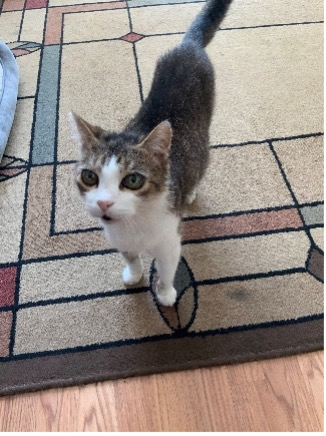
\includegraphics[height=4cm]{btc.jpg}
\caption{The notorious BTC (Brandon The Cat).}
\label{fig:1}
\end{figure}

%%%%%%%%%%%%%%%%%%%%%%%%%%%%%%%%%%%%%%%%%%%%%%%%%%%%%%%%%%%%%%%%%%%%%%%%%%%%%%%%

\chapter{Discussion}
\label{discussion}

\instructions{The discussion section is where you interpret and compare the
results. The objective is to point out the features and limitations of
the work. Relate your results to current knowledge in the field and to
the original purpose for undertaking the project.}

%%%%%%%%%%%%%%%%%%%%%%%%%%%%%%%%%%%%%%%%%%%%%%%%%%%%%%%%%%%%%%%%%%%%%%%%%%%%%%%%

\chapter{Conclusions}
\label{conclusions}

\instructions{This section is written to put the interpretation of the results
into the context of the original problem.~ Do not repeat the discussion
points or include irrelevant material. The conclusion should be based on
the evidence presented.}

%%%%%%%%%%%%%%%%%%%%%%%%%%%%%%%%%%%%%%%%%%%%%%%%%%%%%%%%%%%%%%%%%%%%%%%%%%%%%%%%

\chapter*{References}
\label{references}
\addcontentsline{toc}{chapter}{References}


\instructions{Many bibliographic styles are acceptable for publications 
in the natural sciences. This template uses a numeric style defined in biblatex
and that is common in Physics, Mathematics, and Computer Science papers.}

\printbibliography[heading=none]


%%%%%%%%%%%%%%%%%%%%%%%%%%%%%%%%%%%%%%%%%%%%%%%%%%%%%%%%%%%%%%%%%%%%%%%%%%%%%%%%

\appendix

\chapter{Additional Material}
\label{appendix-a}

This template can be viewed on Overleaf at \url{https://www.overleaf.com/read/hxjcgtkhjqcd}.
If you have an Overleaf account (either free or paid) you can copy this template to start a new Overleaf project.
If you do not want an Overleaf account you can install TeX on your computer and download the template files from Overleaf.

\end{document}